%==================================================
\section{\Cech{} コホモロジー：具体的な計算}\label{sec:cech}
%==================================================

\paragraph{動機。}局所切断を貼り合わせるとき、重なり上の食い違いを記録するのが \Cech{} コホモロジーである。第1巻の Mayer--Vietoris では、二つの開集合による被覆 $M=U\cup V$ で $H^k(U\cap V)\to H^{k+1}(M)$ が現れた。\Cech{} コホモロジーはそれを任意の被覆に一般化したものと思ってよい。計算が具体的なので、まずこれを習熟する。

\subsection{定義}
$\mathcal U=(U_i)_{i\in I}$ を $X$ の開被覆、$\sF$ を層とする。
\begin{defn}[\Cech{} 複体]
$p$ \emph{コチェイン}とは、$I^{p+1}$ の各組 $(i_0,\dots,i_p)$ に $c_{i_0\cdots i_p}\in\sF(U_{i_0\cdots i_p})$ を対応させるもので、\emph{交代的}（添字の置換で符号 $\mathrm{sgn}$ がかかり、添字に重複があれば $0$）なもの。その全体を $C^p(\mathcal U,\sF)$ とし、
\[
(\delta c)_{i_0\cdots i_{p+1}}=\sum_{k=0}^{p+1}(-1)^k\,c_{i_0\cdots\widehat{i_k}\cdots i_{p+1}}\Big|_{U_{i_0\cdots i_{p+1}}}
\]
とおく。$\delta^2=0$。コホモロジー $\check H^p(\mathcal U,\sF)=H^p(C^\bullet(\mathcal U,\sF),\delta)$ を\emph{（被覆 $\mathcal U$ に関する）\Cech{} コホモロジー}という。
\end{defn}
（$I$ に全順序を入れて $i_0<\cdots<i_p$ の組だけで定義しても同じ。交代的な定義の方が細分の扱いが楽なのでこうする。）低次を具体的に書くと：
\begin{itemize}
\item $c=(c_i)\in C^0$：$(\delta c)_{ij}=c_j-c_i$ （$U_{ij}$ 上）。
\item $c=(c_{ij})\in C^1$：$(\delta c)_{ijk}=c_{jk}-c_{ik}+c_{ij}$ （$U_{ijk}$ 上）。したがって $c$ が \emph{1 コサイクル}$\iff c_{ik}=c_{ij}+c_{jk}$（特に $c_{ii}=0$、$c_{ji}=-c_{ij}$）。
\item 1 コボーダリー：$c_{ij}=h_j-h_i$ （$h_i\in\sF(U_i)$）。
\end{itemize}
\begin{prop}\label{prop:cechH0}\tP
$\check H^0(\mathcal U,\sF)=\sF(X)$。
\end{prop}
\begin{proof}
0 コサイクル：$c_j|_{U_{ij}}=c_i|_{U_{ij}}$（すべての $i,j$）。これは (S2) の貼り合わせ条件そのもの。よって $c$ は $s\in\sF(X)$ に貼り合わさり、(S1) から $s$ は一意。逆に $s$ から $c_i=s|_{U_i}$ が得られる。\qedhere
\end{proof}
したがって \Cech{} コホモロジーは「大域切断を $\check H^0$ とみなして、その右側の高次の障害を測る」。群が乗法的な層（$\Oc^*$ など）では、上の式を乗法に読み替える：1 コサイクルの条件 $g_{ik}=g_{ij}g_{jk}$、コボーダリー $g_{ij}=h_j/h_i$。

\subsection{$H^1$ の手計算：円周と定数層}
\begin{ex}[$S^1$、2 枚の弧による被覆]\label{ex:S1cover}
円周 $S^1$ を、2 つの開弧 $U_0,U_1$ で覆う（それぞれ円周から 1 点を除いたもの、二つの除く点 $P,Q$ は異なる）。$U_0\cap U_1$ は 2 つの開弧 $A,B$ の非交和（$P,Q$ の近傍に対応）。定数層 $\Zs$ の \Cech{} 複体：$C^0=\Zs(U_0)\oplus\Zs(U_1)=\Z^2$（各 $U_i$ は連結）、$C^1=\Zs(U_{01})=\Z^2$（$A$ と $B$ の値）、$C^p=0$（$p\ge2$：被覆が 2 枚、交代的）。
\[
\delta(a_0,a_1)=(a_1-a_0\ \text{on}\ A,\ a_1-a_0\ \text{on}\ B)=(a_1-a_0,\ a_1-a_0).
\]
\begin{center}
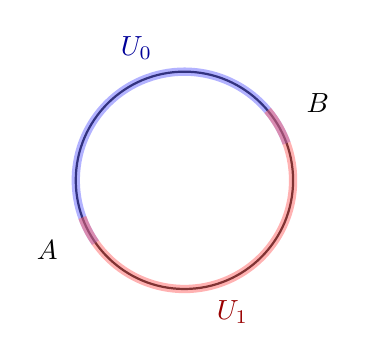
\begin{tikzpicture}[scale=1.15]
\draw[thick] (0,0) circle (1.2);
\draw[line width=3pt,blue!60,opacity=.5] (20:1.2) arc (20:215:1.2);
\draw[line width=3pt,red!60,opacity=.5] (200:1.2) arc (200:400:1.2);
\node[blue!60!black] at (110:1.55) {$U_0$};
\node[red!60!black] at (290:1.55) {$U_1$};
\node at (207:1.7) {$A$};
\node at (30:1.7) {$B$};
\end{tikzpicture}
\end{center}
核は対角 $\{(a,a)\}\cong\Z$（定数関数）、よって $\check H^0=\Z$。像は対角 $\{(m,m)\}$、余核 $\Z^2/\{(m,m)\}\cong\Z$（$(p,q)\mapsto p-q$）。ゆえに
\[
\check H^0(\mathcal U,\Zs)=\Z,\qquad\check H^1(\mathcal U,\Zs)=\Z,\qquad\check H^p=0\ (p\ge2).
\]
生成元はコサイクル $(0\ \text{on}\ A,\ 1\ \text{on}\ B)$：「$A$ では貼り合わせが食い違わず、$B$ では 1 だけずれる」、すなわち普遍被覆 $\R\to S^1$（$\Z$-主束）の貼り合わせデータで、巻き数 1 を表す。$\Z$ を $\R$ に取り替えれば $\check H^1(\mathcal U,\Rs)=\R$、第1巻の $H^1_{\mathrm{dR}}(S^1)=\R$ と一致する（後で de Rham の定理、定理 \ref{thm:deRham}）。
\end{ex}
\begin{ex}[$S^1$、3 枚の弧による被覆]\label{ex:S1three}
$S^1$ を 3 枚の開弧 $U_0,U_1,U_2$（各 $U_i$ は隣と重なり、3 重の交わりは空）で覆う。$U_{01},U_{12},U_{02}$ は各々連結な弧で $U_{012}=\emptyset$。$\Zs$ について、$C^0=\Z^3$、$C^1=\Z^3$（成分 $c_{01},c_{12},c_{02}$）、$C^2=0$。$\delta(a_0,a_1,a_2)=(a_1-a_0,\ a_2-a_1,\ a_2-a_0)$。核は $\{a_0=a_1=a_2\}\cong\Z$、像は階数 2 の部分群（$c_{02}=c_{01}+c_{12}$ をみたす $\{(x,y,x+y)\}$）で、$C^1=\Z^3$ の中で $c_{02}-c_{01}-c_{12}$ の値で測れば余核は $\Z$（$(c_{01},c_{12},c_{02})\mapsto c_{02}-c_{01}-c_{12}$）。したがって $\check H^1=\Z$。2 枚で覆った例 \ref{ex:S1cover} と同じ答え。
\begin{center}
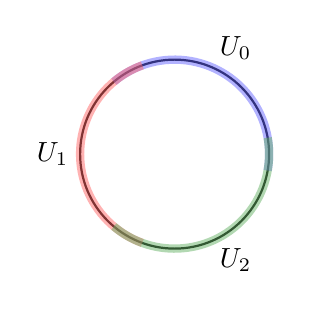
\begin{tikzpicture}[scale=1.0]
\draw[thick] (0,0) circle (1.2);
\foreach \a/\c in {0/blue,120/red,240/green!50!black}{
 \draw[line width=3pt,\c!60,opacity=.5] (\a-10:1.2) arc (\a-10:\a+130:1.2);}
\node at (60:1.55) {$U_0$}; \node at (180:1.55) {$U_1$}; \node at (300:1.55) {$U_2$};
\end{tikzpicture}
\end{center}
\end{ex}
\begin{rem}
この計算は、\Cech{} コホモロジーが（被覆が十分細かければ）位相的な不変量 $H^1(S^1,\Z)=\Z$ を与えることを示している。一般に、各 $U_{i_0\cdots i_p}$ が空か可縮ならば、定数層の \Cech{} コホモロジーは被覆の\emph{神経}（nerve：頂点 $i$、辺 $\{i,j\}$（$U_{ij}\ne\emptyset$）、…の単体複体）の単体コホモロジーに等しい。例 \ref{ex:S1three} はこの条件をみたし、神経は三角形の周（円周）。一方、例 \ref{ex:S1cover} では $U_{01}$ が非連結（2 つの弧）なのでこの条件をみたさない（神経は 1 本の辺で可縮だが、答えの $\check H^1=\Z$ は神経からは出ない）。それでも答えが正しいのは、$H^1(S^1,\Z)=\Z$ と一致しているからで、これは §\ref{sec:leray} の Leray の定理の条件（$U_{01}$ の $H^q(\ ,\Zs)$ が $q\ge1$ で消える）が成り立つため。
\end{rem}

\subsection{細分と極限}
\begin{defn}
$\mathcal V=(V_j)_{j\in J}$ が $\mathcal U$ の\emph{細分}とは、写像 $\tau:J\to I$ で $V_j\subset U_{\tau(j)}$ をみたすものがあること。コチェイン写像 $\tau^*:C^p(\mathcal U,\sF)\to C^p(\mathcal V,\sF)$ を $(\tau^*c)_{j_0\cdots j_p}=c_{\tau(j_0)\cdots\tau(j_p)}|_{V_{j_0\cdots j_p}}$ で定める（$\delta$ と可換）。
\end{defn}
\begin{prop}\tC
コホモロジー上の写像 $\tau^*:\check H^p(\mathcal U,\sF)\to\check H^p(\mathcal V,\sF)$ は、$\tau$ の選び方によらない。
\end{prop}
\src{Hartshorne, 第III章 演習 4.4(a)(b)（細分写像と、$\check H^p(\mathcal U,\sF)\to H^p(X,\sF)$ との整合。演習番号は確認済）。Godement, 第II章（\Cech{} コホモロジーの節、節番号は\tQ{}）。}
このため $\check H^p(X,\sF)=\varinjlim_{\mathcal U}\check H^p(\mathcal U,\sF)$（細分に関する帰納極限）が定まる（\emph{\Cech{} コホモロジー}）。
\begin{prop}\label{prop:H1inj}\tP
$\mathcal V$ が $\mathcal U$ の細分のとき、$\tau^*:\check H^1(\mathcal U,\sF)\to\check H^1(\mathcal V,\sF)$ は単射である。したがって $\check H^1(\mathcal U,\sF)\hookrightarrow\check H^1(X,\sF)$。
\end{prop}
\begin{proof}
問 \ref{p:refinj} で証明する（コサイクル $c$ に対し $\tau^*c=\delta h$ とする。$V_j\subset U_{\tau(j)}$ 上で $h_j$ を、$x\in U_i$ の近傍で $h_j$ から $\sF(U_i)$ の元を貼り合わせて作る）。\qedhere
\end{proof}
\begin{thm}\tC
任意の位相空間 $X$、層 $\sF$ について、\Cech{} の $\check H^1(X,\sF)$ は \S\ref{sec:cohom} で定義する層コホモロジー $H^1(X,\sF)$ に自然に同型。（$H^2$ 以上では一般に一致しない。paracompact Hausdorff 空間では全次数で一致する。）
\end{thm}
\src{Hartshorne, 第III章 演習 4.4(c)（任意の位相空間で $\varinjlim_{\mathcal U}\check H^1(\mathcal U,\sF)\to H^1(X,\sF)$ が同型。確認済）。paracompact Hausdorff での全次数の一致：Godement, 第II章（節番号は\tQ{}）。}

\subsection{Mayer--Vietoris の形}
被覆が 2 枚 $\mathcal U=\{U,V\}$ のとき、$C^0=\sF(U)\oplus\sF(V)$、$C^1=\sF(U\cap V)$、$C^p=0$（$p\ge2$）。$\delta(a,b)=b|_{U\cap V}-a|_{U\cap V}$。したがって
\[
0\to\check H^0(\mathcal U,\sF)\to\sF(U)\oplus\sF(V)\xrightarrow{\ \delta\ }\sF(U\cap V)\to\check H^1(\mathcal U,\sF)\to0
\]
は完全で、$\check H^0=\sF(X)$（命題 \ref{prop:cechH0}）。\emph{$\check H^1(\{U,V\},\sF)$ は、$\sF(U\cap V)$ のうち「$\sF(U)$ の元と $\sF(V)$ の元の差」の形に書けないものの全体}である。これが第1巻の Mayer--Vietoris $H^k(U)\oplus H^k(V)\to H^k(U\cap V)\xrightarrow{\delta}H^{k+1}(M)$ の（$k=0$ のときの）層論的な形。以後の \S\ref{sec:leray} の $\CP^1$ の計算は、この形で行う。

\subsection{直線束と $H^1(X,\Oc^*)$}
複素多様体 $X$ 上の正則直線束の同型類全体を $\Pic(X)$ と書く（テンソル積について群をなす：単位元は自明束、逆元は双対束）。
\begin{thm}\label{thm:picH1}\tP
$\Pic(X)\cong\check H^1(X,\Oc^*)$（群の同型。右辺は乗法的な層 $\Oc^*$ の \Cech{} コホモロジー）。直線束のテンソル積はコサイクルの積に、双対はコサイクルの逆元に対応する。
\end{thm}
\begin{proof}
\emph{(1) 直線束からコサイクル。}$L$ を正則直線束とし、$X$ の開被覆 $\mathcal U=(U_i)$ と、各 $U_i$ 上の零点をもたない正則切断（局所枠）$e_i\in L(U_i)$ をとる（$L$ が $U_i$ 上自明になる被覆）。$U_{ij}$ 上で $e_j=g_{ij}e_i$ と書け、$g_{ij}\in\Oc^*(U_{ij})$。（切断 $\sigma=f_ie_i=f_je_j$ の成分は $f_i=g_{ij}f_j$。第1巻の規約と同じ。）$U_{ijk}$ 上 $e_k=g_{ik}e_i$、かつ $e_k=g_{jk}e_j=g_{jk}g_{ij}e_i$ より $g_{ik}=g_{ij}g_{jk}$：$g=(g_{ij})$ は 1 コサイクル。別の枠 $e_i'=h_ie_i$（$h_i\in\Oc^*(U_i)$）では $e'_j=h_jg_{ij}h_i^{-1}e'_i$ なので $g'_{ij}=g_{ij}\cdot(h_j/h_i)$：コボーダリーだけ変わる。別の被覆では共通細分をとって比べる。こうして類 $[L]\in\check H^1(X,\Oc^*)$ が定まる。同型な直線束は同じ類を与える（同型で枠を写す）。

\emph{(2) 単射。}$L,L'$ が同じ類をもてば、共通の被覆と枠 $e_i,e'_i$ について $g'_{ij}=g_{ij}\,h_j/h_i$（$h_i\in\Oc^*(U_i)$）と書ける。$\phi:L|_{U_i}\to L'|_{U_i}$ を $\phi(e_i)=h_i^{-1}e'_i$ で定める。$U_{ij}$ 上で $\phi(e_j)=h_j^{-1}e'_j=h_j^{-1}g'_{ij}e'_i=g_{ij}h_i^{-1}e'_i=g_{ij}\phi(e_i)$ となり、これは $e_j=g_{ij}e_i$ の $\phi$ による像と一致する。よって $\phi$ は貼り合わさって同型 $L\cong L'$ を与える。

\emph{(3) 全射。}コサイクル $g=(g_{ij})$ が与えられたら、$E=\bigsqcup_iU_i\times\C/\sim$、$(x,v)_j\sim(x,g_{ij}(x)v)_i$（$x\in U_{ij}$）で束を作る。コサイクル条件 $g_{ik}=g_{ij}g_{jk}$ が同値関係であること（推移律）を保証する。局所枠 $e_i=[(x,1)_i]$ に対し $e_j=g_{ij}e_i$ をみたすから、$[E]=[g]$。コボーダリーの違いは (2) より同型。

\emph{(4) 準同型。}$L\otimes L'$ は枠 $e_i\otimes e_i'$ をもち、$e_j\otimes e_j'=g_{ij}g'_{ij}\,e_i\otimes e_i'$。双対束は双対枠で $g_{ij}^{-1}$。\qedhere
\end{proof}
\begin{ex}[$\Oc(k)\to\CP^1$ のコサイクル]\label{ex:Okcocycle}
\S\ref{sec:examples} の規約（$\sigma=f_0e_0=f_1e_1$、$f_1=z^{-k}f_0$）では $e_1=z^ke_0$：被覆 $\{U_0,U_1\}$ で $g_{01}=z^k\in\Oc^*(U_{01})=\Oc^*(\C^*)$。$\Oc(k)\otimes\Oc(l)=\Oc(k+l)$（$z^kz^l=z^{k+l}$）、$\Oc(k)^*=\Oc(-k)$。$\Oc(-1)$ では $e_1=z^{-1}e_0$（第2巻の $e_0=ze_1$ と同じ）。標準束 $K=\Omega^1_{\CP^1}$：$U_0$ の枠 $dz$、$U_1$ の枠 $dw=-z^{-2}dz$ より $g_{01}=-z^{-2}$。$-1=e^{\pi i}$ と書けば $-z^{-2}=z^{-2}\cdot(-1)$ で、定数 $-1\in\Oc^*(U_0)$ で割る（$h_0=-1,h_1=1$ の取り替え）と $g_{01}'=z^{-2}$：$K\cong\Oc(-2)$。
\end{ex}
\begin{prop}\label{prop:Oknontriv}\tP
$k\ne l$ ならば $\Oc(k)\not\cong\Oc(l)$。特に $\Oc(k)$ $(k\ne0)$ は自明でない。
\end{prop}
\begin{proof}
$\Oc(k)\cong\Oc(l)$ なら $\Oc(k-l)$ が自明（$\Oc(k)\otimes\Oc(l)^*$）。$m=k-l$ とし、$\Oc(m)$ が自明と仮定する。コサイクル $g_{01}=z^m$ がコボーダリー $h_1/h_0$ に等しい：$z^m=h_1(z)/h_0(z)$（$h_0\in\Oc^*(\C)$、$h_1\in\Oc^*(\C\setminus0\ \text{を}\ w=1/z\ \text{で見て}\ \C_w)$、すなわち $h_1(z)=\tilde h_1(1/z)$、$\tilde h_1\in\Oc^*(\C_w)$）。単位円周 $|z|=1$ をまわる偏角の変化（巻き数）をとる。$h_0$ は $|z|\le1$ で零点をもたない正則関数なので、偏角の原理から $h_0(e^{i\theta})$ の巻き数は $0$。$\tilde h_1$ は $|w|\le1$ で零点をもたない正則関数なので、$\tilde h_1(e^{-i\theta})$ の巻き数も $0$（$|w|=1$ をどちら向きに回っても $0$）。一方 $z^m$ の巻き数は $m$。よって $m=0$。\qedhere
\end{proof}
（$\Pic(\CP^1)\cong\Z$ であること、すなわち \emph{すべての}直線束が $\Oc(k)$ であることは、§\ref{sec:leray} で示す。）

\begin{keybox}{要点（§\ref{sec:cech}）}
\Cech{} 複体は、被覆の重なり上の切断の組（0 コチェイン、1 コチェイン、…）と、交代和の $\delta$。$\check H^0=$ 大域切断、$\check H^1=$ 貼り合わせの食い違いの類（Mayer--Vietoris の形）。$\check H^1(X,\Oc^*)=\Pic(X)$。$\Oc(k)$ のコサイクルは $g_{01}=z^k$。被覆の取り方に依存するのが弱点で、それを細分の極限（または Leray の定理）で解決する。
\end{keybox}

\begin{prob}{基本}\label{p:S1cech}
$S^1$ を 3 枚の弧で覆う（例 \ref{ex:S1three}）。層 $\Zs$ の \Cech{} 複体 $0\to C^0\to C^1\to0$ を書き下し、$\check H^0=\Z$、$\check H^1=\Z$ を確かめよ。1 コサイクル $(c_{01},c_{12},c_{02})=(0,0,1)$ が生成元であること、また、これは $a_i$ でコボーダリーとして書けないことを直接確かめよ。
\end{prob}
\begin{prob}{標準}\label{p:S2cech}
$S^2$ を上半球 $U_0$ と下半球 $U_1$（それぞれ少しずつ開いてのばし、$U_0\cap U_1$ は赤道を含む帯状領域）で覆う。(a) $\check H^1(\{U_0,U_1\},\Zs)=0$ を示せ。(b) $H^2(S^2,\Z)=\Z$（位相的な事実）であるのに、この被覆の \Cech{} $\check H^2$ は $0$ である。なぜ矛盾しないか。（ヒント：$U_{01}$ は円周と同ホモトピーで、$H^1(U_{01},\Zs)\ne0$。Leray の被覆の条件、定理 \ref{thm:leray}。）
\end{prob}
\begin{prob}{基本}\label{p:cocycleOk}
$\CP^1$ の被覆 $\{U_0,U_1\}$ で、$\Oc(3)\otimes\Oc(-5)$ のコサイクルを書け。それが $\Oc(-2)$ のコサイクルと一致すること、また $K_{\CP^1}$ のコサイクル $-z^{-2}$ と $z^{-2}$ がコボーダリーで結ばれること（例 \ref{ex:Okcocycle}）を確かめよ。
\end{prob}
\begin{prob}{標準}\label{p:moebius}
$S^1$ の被覆 $\{U_0,U_1\}$（例 \ref{ex:S1cover}）と、符号 $\{\pm1\}$ の定数層 $\underline{\{\pm1\}}$ を考える。(a) $\check H^1(\mathcal U,\underline{\{\pm1\}})\cong\Z/2$ を示せ。(b) 非自明な類に対応する実直線束は Möbius 束で、自明な類は自明束であることを、貼り合わせ関数 $g_{01}\in\{\pm1\}$（$A$ 上 $+1$、$B$ 上 $-1$）から説明せよ。
\end{prob}
\begin{prob}{発展}\label{p:refinj}
命題 \ref{prop:H1inj} を証明せよ。（ヒント：$\tau:J\to I$ を細分写像、$c\in C^1(\mathcal U,\sF)$ を 1 コサイクルとし、$\tau^*c=\delta h$（$h_j\in\sF(V_j)$）と仮定する。各 $i$ について、$U_i\cap V_j$ 上の切断 $h_j+c_{\tau(j)i}$ を考え、$U_i\cap V_{jl}$ 上で $j,l$ について一致することをコサイクル条件で示す。貼り合わせて $k_i\in\sF(U_i)$ を得て $c=\delta k$ を示せ。）
\end{prob}
\begin{prob}{標準}\label{p:H1oneforms}
\Cech{} $\check H^1(\mathcal U,\Cs)$（$X=\C^*$、$\mathcal U=\{U_1,U_2\}$ は例 \ref{ex:notsheaf}(3) の被覆）を計算し、$\C$ と同型であることを示せ。$H^1_{\mathrm{dR}}(\C^*;\C)=\C$ との対応で、生成元は閉形式 $\frac{1}{2\pi i}\frac{dz}{z}$ に対応する。どのコサイクルか。
\end{prob}

